\documentclass[a4paper]{article}
\usepackage[utf8]{inputenc}
\usepackage[english]{babel}
\usepackage[babel=true]{csquotes}
\usepackage{graphicx}
\usepackage[cm]{fullpage}
\usepackage{multirow}

\pagestyle{headings}

\title{Programming techniques : Project 3}
\author{Raphaël Javaux}
\date{}

\begin{document}

\maketitle

   \subsection{Sequential optimisations}

   \subsubsection{Neighbourhood coordinates lookup tables}

    \paragraph{}To avoid to compute the neighbours coordinates in the
\textit{toroidal square world} at each iteration, I used two lookup tables to
precompute the coordinates of, respectively, the previous column/row and the
next column/row for each column/row. This gave an \textbf{1.4x} speedup to the
algorithm by removing four conditional expressions.

   \subsubsection{Board of bytes instead of booleans}

   \paragraph{}By storing the game's board state in an array of \textit{bytes},
with cells labelled with \textit{1} for \textit{alive} and \textit{0} for
\textit{dead}, I was able to replace the inspection of cell status by an eight
terms addition, removing as many conditional expressions. This gave me an
additional \textbf{5x} speedup.

  \subsection{Programming languages}

    \paragraph{}In addition to the required Java tests, I written my
\textbf{sequential} generation algorithm in two additional programming
languages :
    \begin{itemize}
        \item In \textit{C} because of its very competitive compilers (GCC 4.8
was used) and the similar syntax to Java which enabled me to almost copy-paste
the algorithm ;
        \item In \textit{Haskell} because this functional language provides
automatic and deterministic array parallelisation (parallelisation of a function
is a compile time option and is guaranteed by the compiler to give the same
result as the sequential execution).
    \end{itemize}
Both versions implements exactly the same algorithm as the Java sequential one,
except that the Haskell's is able to execute itself in parallel automatically.

  \section{Results}

    \paragraph{}These results have been collected on a dual Intel 2Ghz
haxa-cores hyper-threaded machine, giving 24 logical cores for 12 physical
cores. Each of the following results is obtained by  computing the mean
execution time of an hundred repeated executions. As the naive strategy (spawn
a new thread for each cell) wasn't able to scale up to a board of more than
a thousand cells, it was removed from my tests.

    \paragraph{}Figure \ref{fig:10080_throughput} shows the number of cells
which can be generated per second by each method given a certain amount of
threading on a large board. Notice that the block segmentation is only able to
use square numbers of threads and that the board size must also be a multiple of
144 (the LCM of 1, 4, 9 and 16). \newline
The sequential C algorithm is awfully fast, probably because the C compiler is
smart enough to use vectorial instructions while others aren't.\newline
The linear segmentation is the most effective parallel strategy (it's also the
one used by Haskell internally). The column segmentation is deadly ineffective
because of being cache unfriendly. Haskell scales in an almost perfect speedup
until reaching the number of physical cores, which makes me hint that the
benchmark is not bounded by the memory bandwidth, even on this 24-cores machine.

    \begin{figure}[h]
        \centering
        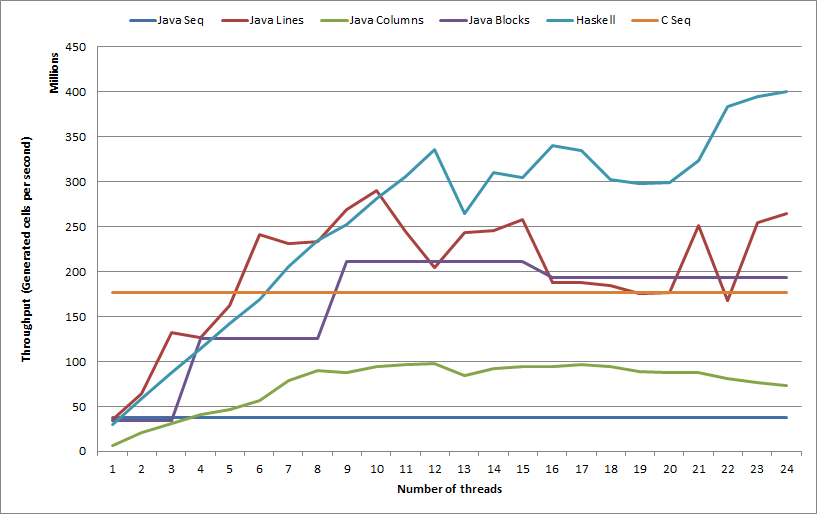
\includegraphics[width=0.7\linewidth]{results/10080_throughput.png}
        \caption{
            Cell generation rate on a 10,080 x 10,080 board
            \label{fig:10080_throughput}
        }
    \end{figure}

    \paragraph{}Figure \ref{fig:board_size_impact} shows the impact of different
board sizes on the cell throughput, given the most efficient number of threads
for each method for each size. \newline
The performance index is calculated for each method by comparing the best
performance obtained to the speed of the sequential Java implementation.
Parallel implementations shine as well as the number of cells in the board
increase. The sequential C implementation almost loose half its speed when the
size of the board exceeds the CPU cache whereas the sequential Java
implementation has stable, but poor, performances.

    \begin{figure}[h]
        \centering
        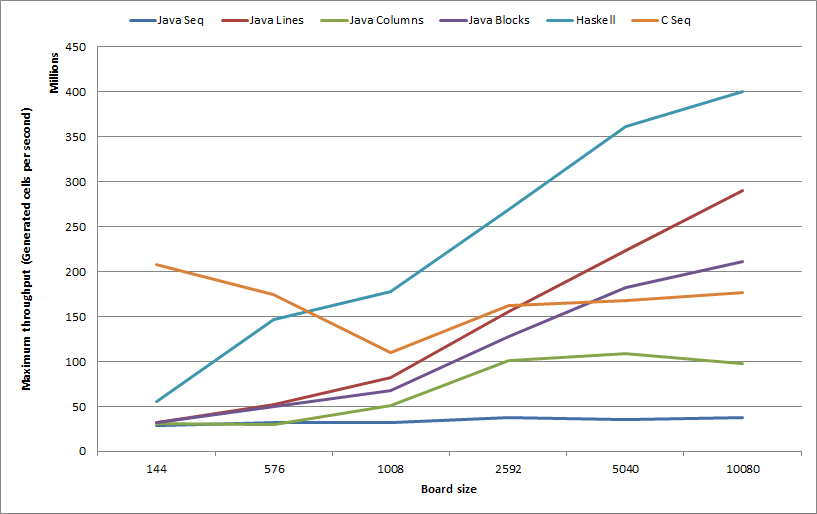
\includegraphics[width=0.7\linewidth]{results/board_size_impact.png}

        \begin{tabular}{  ll | l  l  l  l  l  l }
            & & 144 & 576 & 1008 & 2592 & 5040 & 10080 \\ \hline

            Java Seq & Performance index & 1 & 1 & 1 & 1 & 1 & 1 \\
            Java Lines
                & Performance index & 1 & 1.6 & 2.6 & 4.2 & 6.3 & 7.8 \\
                & Parallel speedup  & 1 & 1.4 & 2.5 & 4.3 & 6.5 & 8.1 \\
                & Threads           & 1 & 5   & 9   & 9   & 6   & 10 \\
            Java Columns
                & Performance index & 1 & 0.9 & 1.6 & 2.7 & 3.1 & 2.6 \\
                & Parallel speedup  & 1 & 1   & 2   & 5   & 8.8 
                                    & \textbf{14.5} \\
                & Threads           & 1 & 1   & 8   & 7   & 11  & 11 \\
            Java Blocks
                & Performance index & 1 & 1.6 & 2.1 & 3.4
                                    & 5.1 & 5.7 \\
                & Parallel speedup  & 1 & 1.4 & 2.1 & 3.7
                                    & 5.6 & 6.1 \\
                & Threads           & 1 & 4   & 4   & 9
                                    & 9 & 15 \\
            Haskell
                & Performance index & 1.9 & 4.6
                                    & \textbf{5.5}  & \textbf{7.2}
                                    & \textbf{10.1} & \textbf{10.7} \\
                & Parallel speedup  & \textbf{2.3}  & \textbf{9.7}
                                    & \textbf{7.2}  & \textbf{9.1}
                                    & \textbf{12.2} & 13.3 \\
                & Threads           & \textbf{4}    & \textbf{18}
                                    & \textbf{22}   & \textbf{20}
                                    & \textbf{24}   & \textbf{24} \\
            C Seq & Performance index & \textbf{7.1} & \textbf{5.5}
                                      & 3.4 & 4.4 & 4.7 & 4.7 \\
        \end{tabular}

        \caption{
            Maximum cell generation rate on different board sizes
            \label{fig:board_size_impact}
        }
    \end{figure}

\end{document}